\documentclass{beamer}

\usepackage{Style/transparents}

\title{ASR2-Système : ordinateurs et systèmes d'exploitation}
      
\author{Semestre 2, année 2011-2012}
\institute{
  Département d'Informatique\\
  IUT Bordeaux 1
}
\date{Avril 2012}
    
% Effacer cela si vous ne voulez pas que la table des matières 
% apparaîsse au début de chaque section
% \AtBeginSection[] {
%   \begin{frame}<beamer>
%     \frametitle{Plan}
%     \tableofcontents[currentsection,currentsubsection]
%   \end{frame}
% }

% --------------------------------------------------------------

\begin{document}  

\begin{frame}
  \titlepage
\end{frame}

\begin{frame}
  \frametitle{Introduction aux systèmes d'exploitation}
  \tableofcontents
\end{frame}

  
  % -- et c'est parti

\section{Qu'est-ce qu'un système d'exploitation ?}
\subsection{Définition}

\begin{frame}
  \frametitle{Qu'est-ce qu'un système d'exploitation ?}
  
  \begin{block}{Système d'exploitation}
    \begin{itemize}
    \item programme qui permet d'exploiter les ressources matérielles
    \item fournit \alert{au programmeur d'application} un
      environnement avec facilité d'emploi et utilisation efficace des
      ressources.
    \end{itemize}
  \end{block}
\end{frame}

\subsection{Intérêt}

\begin{frame}
  \frametitle{Facilité d'emploi} 
  
  Le système d'exploitation cache les détails matériels
  sous une \alert{couche
    d'abstraction.}
\vfill  
Il fournit une API (Application Programming Interface) pour utiliser les
ressources.
\vfill
  \begin{block}{Exemples}
    \begin{itemize}
    \item communication réseau par différents moyens
    \item utilisation de fichiers sur différents supports, à travers le réseau, etc.
    \item ...
    \end{itemize}
  \end{block}
\end{frame}
  
\begin{frame}
  \frametitle{Utilisation des ressources} 
  
  Le système d'exploitation est un
  \alert{gestionnaire de ressources} ; il gère l'allocation 
  \begin{itemize}
  \item des
    processeurs, 
      \item de la mémoire,
	\item des périphériques 
	\item etc.
  \end{itemize}

  \structure{Attention}, ne pas confondre système d'exploitation et
  interface utilisateur !

\end{frame}


\subsection{Évolution}


\begin{frame}[containsverbatim]
\frametitle{Évolution des systèmes d'exploitation}
\begin{multicols}{2}
L'histoire des systèmes d'exploitation est liée
à 
\begin{itemize}
\item l'évolution des matériels
\item la manière de les utiliser
\end{itemize}

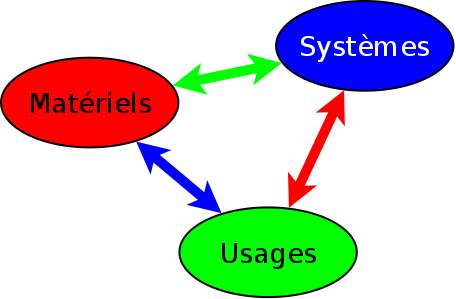
\includegraphics[width=0.9\linewidth]{Figures/materiels-systemes-usages.png}
\end{multicols}

\end{frame}


\begin{frame}
\frametitle{Période charnière}
Les idées fondamentales ont été inventées et mises en oeuvre 
entre
\begin{itemize}
\item \alert{1948} : le premier ordinateur
\item \alert{1964} : les systèmes multitâches en temps partagé (CTSS)
\item \alert{1967} : la virtualisation (CP-67, d'IBM)
\end{itemize}
\end{frame}


\section{Le premier ordinateur : SSEM (Manchester, 1948)}

\begin{frame}
\frametitle{Le premier ordinateur :  SSEM}


\begin{center}
% http://www.computinghistory.org.uk/userdata/files/1_history-ssem.jpg
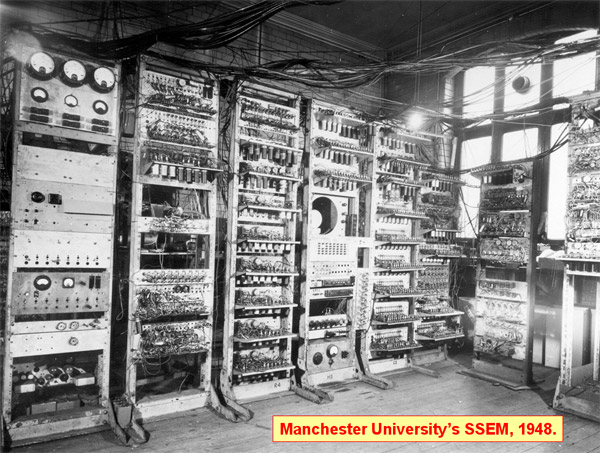
\includegraphics[width=0.75\linewidth]{Historique/1_history-ssem.jpg}
\end{center}

\alert{Small Scale Experimental Machine} , alias ``Baby'' (\alert{21 juin 1948}),

\end{frame}

\begin{frame}
\frametitle{Le premier ordinateur}

\begin{itemize}
\item  calculateur électronique à \alert{programme enregistré}

\item  Tom \alert{Kilburn}, Geoff \alert{Tootill}, et Fred. \alert{Williams}, université de Manchester

\item Tourne la première fois le 21 juin 1948


\item Video
\url{http://news.bbc.co.uk/2/hi/technology/7465115.stm}
\end{itemize}

\end{frame}


\begin{frame}

\frametitle{Objectifs du SSEM}

\begin{multicols}{2}
\alert{Objectifs}
\begin{itemize}
\item machine \alert{expérimentale}
\item test de la  mémoire à \alert{tube de Williams-Kilburn}
\item \alert{utilisabilité ?}
\end{itemize}

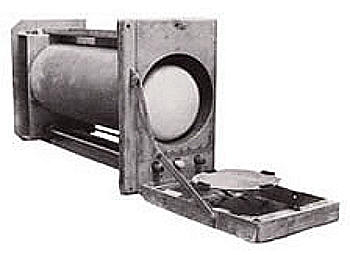
\includegraphics[width=\linewidth]{Historique/william-kilburn_tube.jpg}

\end{multicols}
\end{frame}

\begin{frame}
\frametitle{Tube de Williams-Kilburn}

\begin{block}{Ecriture}
\begin{itemize}
\item \alert{tube cathodique} : un faisceau d'électrons ``allume'' des points
de phosphore sur un écran ( 
\item Pilotage du faisceau en X,Y = accès direct
\end{itemize}
\end{block}

\begin{block}{Lecture}
\begin{itemize}
\item \alert{point déjà allumé} : émet des électrons secondaires
\item \alert{détection par une plaque} devant l'écran
\end{itemize}
\end{block}

\end{frame}
\begin{frame}
\frametitle{Réalisation}

\begin{multicols}{2}

\alert{Réalisation}
\begin{itemize}
\item Machine 32 bits, mémoire de 32 mots (ext. à 2048).
\item Deux registres : Accumulateur, Compteur de Programme, Registre d'Instruction
\item Jeu de 7 instructions
\end{itemize}
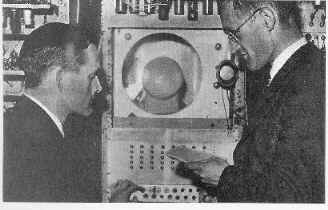
\includegraphics[width=0.9\linewidth]{Historique/hist409t.jpg}
\end{multicols}

\end{frame}

\begin{frame}
\frametitle{Contexte (1948)}

\begin{itemize}
\item depuis la fin du XIXe, machines mécanographiques (cartes perforées) pour 
le traitement de l'information
\item en 1948 les calculateurs électroniques existaient  
\begin{itemize}
\item
  \alert{Z3} de Konrad Zuse en \alert{1942} (relais)
\item \alert{Colossus}, Tommy Flowers, \alert{1943}  (1500 tubes à vide)
 \item \alert{ENIAC} d'Eckert et Mauchly, \alert{1946} (17500 tubes)
\end{itemize}
\end{itemize}
\end{frame}

\begin{frame}
\frametitle{Contexte (1948)}

\begin{itemize}
\item  calculateurs à \alert{programmes externes}
  \begin{itemize}
    \item sur \alert{bande perforée}
      \item \alert{tableau de prises} à enficher
\end{itemize}
\item technologies \alert{trop lentes} ou \alert{trop chères} pour le stockage des programmes
\begin{itemize}
\item tubes à vide
\item lignes à retard (mercure)
\end{itemize}
\end{itemize}
\end{frame}

\begin{frame}
\frametitle{Du tube de Williams-Kilburn au SSEM}

\begin{itemize}
\item En 1947, W et K arrivent à stocker 2048 bits sur un écran d'oscilloscope
\item technologie performante et ``bon marché''
\item tests manuels ne permettent pas de s'assurer de la fiabilité
\item donc \alert{décision de réaliser un calculateur expérimental}
\end{itemize}
\end{frame}


\begin{frame}
\frametitle{Succès}
\begin{itemize}
\item calcul du plus grand diviseur propre de $2^{18}$ 
\item programme de 17 instructions
\item divisions par soustraction successives
\item 52 minutes de calcul, 
\item 3,5 millions d'instructions, environ 1100 instr/seconde
\item résultat = .... ?
\end{itemize}
\end{frame}

\subsection{SSEM : éléments}
\begin{frame}
\frametitle{SSEM : éléments}
\begin{multicols}{2}
\begin{itemize}
\item mémoire 32 mots de 32 bits (M), sert d'affichage
\item 3 registres 
\begin{itemize}
\item \alert{current instruction} (CI) : 11 bits, numéro de l'instruction en cours
\item \alert{program instruction} (PI) : 32 bits, instruction en cours
\item \alert{accumulateur} (A) : 32 bits.
\end{itemize}
\item bit AUTO (marche/arrêt)
\item additionneur/soustracteur
\end{itemize}
\begin{center}
% http://en.wikipedia.org/wiki/File:BabyArchitecture.png
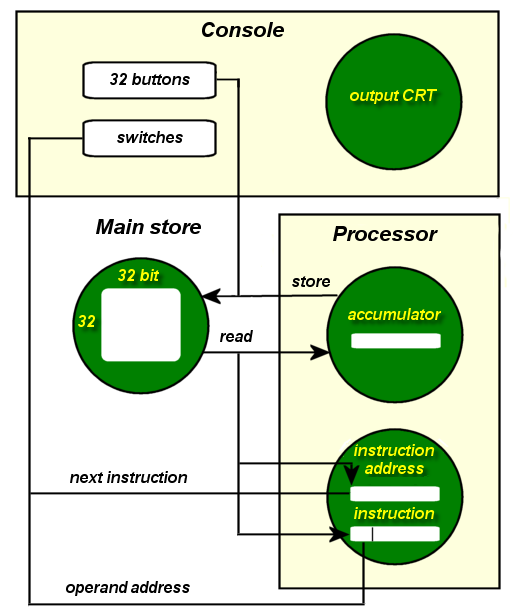
\includegraphics[width=\linewidth]{Historique/BabyArchitecture.png}
\end{center}

\end{multicols}
\end{frame}


\subsection{Cycle de fonctionnement}
\begin{frame}
\frametitle{SSEM : Cycle de fonctionnement} 

\begin{multicols}{2}
si AUTO = 1, le processeur exécute des cycles :
\begin{enumerate}
\item \texttt{PI = M[CI]} recherche de l'instruction (\alert{FETCH})
\item exécution de l'instruction dans PI (\alert{EXECUTE})
\item \texttt{PI = PI+1}
\end{enumerate}
\begin{center}
% http://en.wikipedia.org/wiki/File:BabyArchitecture.png
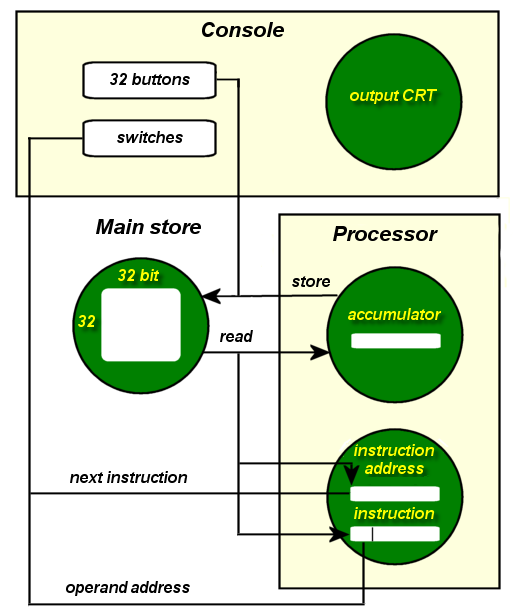
\includegraphics[width=\linewidth]{Historique/BabyArchitecture.png}
\end{center}
\end{multicols}
\end{frame}

\subsection{Jeu d'instructions du SSEM}
\begin{frame}
\frametitle{Les instructions du SSEM}

Les instructions sur 32 bits contiennent
\begin{itemize}
\item Un \alert{code opération} F sur 3 bits
\item Une \alert{adresse} S sur 11 bits
\end{itemize}

\vfill 
\begin{tabular}{|l|l|l|l|}
\hline
F (3) &  (2) & S (11)  &  (16) \\
\hline
f f f  & - - & s s s s s s s s s s s & - - - - - - - - - - - - - - - - \\
\hline
\end{tabular}

\vfill
Les autres bits sont ignorés.
\end{frame}

\begin{frame}
\frametitle{Jeu d'instructions}

Seulement 7 instructions :
\vfill
\begin{tabular}{|c|c|l|l|}
\hline
F & nom & effet & description  \\
\hline
000 & JMP &  \texttt{CI = M[S]} & saut indirect \\
001 & SUB &  \texttt{A -= M[S]} & soustraction \\
010 & LDN &  \texttt{A = -M[S]} & chargement de l'opposé \\
011 & CMP &  si A négatif,  \texttt{CI++} & saute instruction si A négatif \\
100 & JPR &  \texttt{CI += M[S]} & saut relatif \\
101 & - & - & - \\
110 & STO &  \texttt{M[S] = A} & rangement \\
111 & HLT &  \texttt{AUTO = 0} & arrêt \\
\hline 
\end{tabular}
\vfill
Pas d'addition ?
\end{frame}

\subsection{Programmation}
\begin{frame}[containsverbatim]
\frametitle{Exemple de programme : addition de deux nombres }
Calcule \texttt{Z = X + Y},
avec X, Y et Z situées en 20, 21, 22

\begin{verbatim}
num  instruction  effet
---   ----------  -----------------------
  0   LDN 20      A contient -X
  1   SUB 21      A contient -X-Y = -(X+Y) 

  2   STO 22      Z contient -(X+Y)
  3   LDN 23      A contient X+Y

  4   STN 23      Z contient X+Y
  5   HLT         arrêt
\end{verbatim}

en \alert{langage d'assemblage} (anachronique)

\end{frame}

\subsection{Et ensuite ?}
\subsubsection{Évolution des technologies (mémoire)}
\begin{frame}
\frametitle{Les suites du SSEM : technologies}

\begin{itemize}
\item Les tubes de Williams ont été utilisés dans quelques machines
(IBM 701, 1953)
\item technologie abandonnée peu après au profit des \alert{tores de ferrite},
utilisés entre 1955 et 1975.
\item L'université de Manchester a développé le \alert{premier ordinateur à
  transistors} (1953). 
\end{itemize}
\end{frame}

\subsubsection{Évolution des technologies (processeurs)}

\begin{frame}
\frametitle{Machines à transistors}

Invention du transistor
\begin{itemize}
\item à effet de champ  en 1925, et oublié...
\item bipolaire à points de contact, en 1947 (Shockley, Bardeen et Brattain)
\end{itemize}

IBM 608 (1957) première machine entièrement
  transistorisée : seconde génération.

\end{frame}

  \begin{frame}


\frametitle{Les suites du SSEM (machines)}

\begin{itemize}
\item
Le SSEM a posé les bases de l'architecture des machines modernes 


\item l'université de Manchester a développé (avec Ferranti) des
  ordinateurs, commercialisés à partir de 1951 :
\item Mark 1, sur lequel ont tourné
  tourné
\begin{itemize}
\item le premier programme de musique
\item le premier programme de jeu (résolution de problèmes d'échec,
  mat en deux coups)
\end{itemize}
\item les premiers super-calculateurs : ATLAS / ATLAS 2 / TITAN 
\end{itemize}
\end{frame}

\section{Architecture des ordinateurs}
\begin{frame}
On retrouve les mêmes principes dans tous les ordinateurs.
\begin{itemize}
\item processeur
\item mémoire
\item périphériques
\end{itemize}

Ce qui peut changer, dans le processeur :
\begin{itemize}
\item la taille des mots
\item les registres
\item les instructions
\item les modes d'adressages
\item ...
\end{itemize}
\end{frame}

\subsection{Exemple d'architecture : Intel 8080}
\begin{frame}
\frametitle{Architecture d'un processeur : 8080 Intel (1974)}

\begin{center}
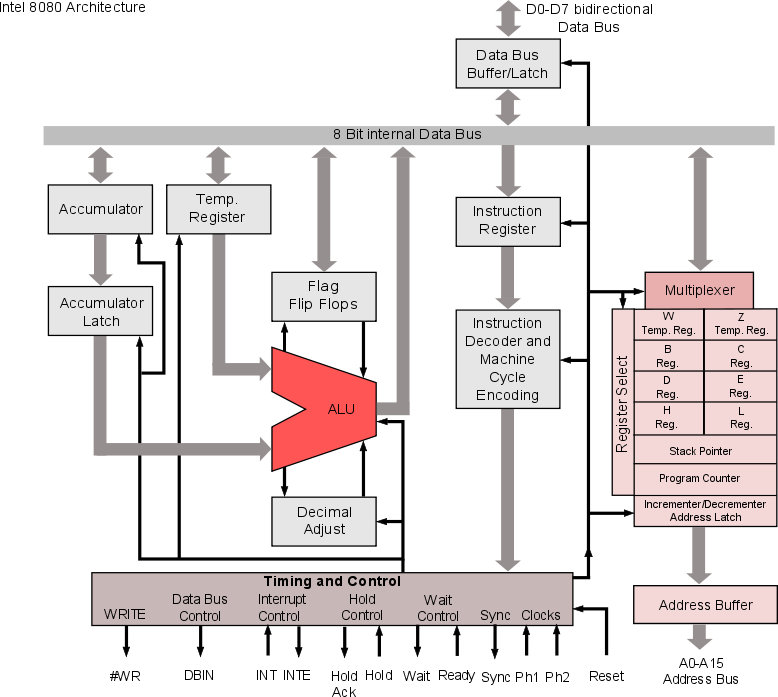
\includegraphics[width=0.7\linewidth]{Historique/8080.png}
\end{center}
\end{frame}

\begin{frame}
\frametitle{Architecture d'un processeur : 8080 Intel (1974)}

\begin{multicols}{2}
\frametitle{Architecture du 8080}
On retrouve
\begin{itemize}
\item accumulateur (8 bits)
\item compteur de programme (16 bits)
\item unité arithmétique et logique
\item registre d'instruction
\item bus de données et d'adresses
\item registres généraux
% \item chemins de données
\item ...
\end{itemize}
r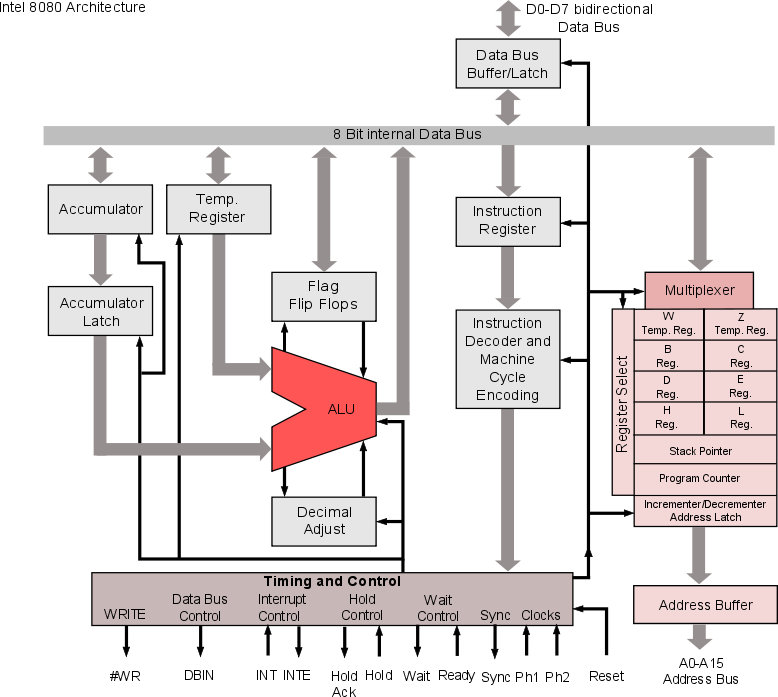
\includegraphics[width=\linewidth]{Historique/8080.png}

\end{multicols}
\end{frame}

\section{Les générations d'ordinateurs}
\begin{frame}
  \frametitle{Générations d'ordinateurs}

  \begin{tabular}{|cll|}
\hline
    \structure{Génération} & \structure{Période} & \
structure{Technologies et machines} \\
    \hline    \hline
Première & 1945-1955 & \alert{tubes à vide} \\
\hline
Seconde & 1955-1965  & machines à \alert{transistors} \\
& & mini-ordinateurs : PDP-1 de DEC (1960)\\
& & 4 kilo-mots de 18 bits, 120.000 \$ \\
\hline
Troisième  &  1965-1971 & \alert{circuits intégrés} \\
 & & Gamme System/360 d'IBM (1966) \\
\hline
Quatrième & 1971-... & \alert{circuits VLSI,
micro-processeurs}. \\
\hline
  \end{tabular}
\end{frame}




\section{Évolution des usages}

\begin{frame}
  \frametitle{ Évolution des usages et des systèmes}

\begin{center}
\begin{tabular}{|l|l|}
\hline
\structure{Type d'usage} & \structure{Type de système}  \\
\hline \hline
Un programme à la fois & - \\
\hline
Enchaînement & moniteur  \\
 automatique & résident  \\
\hline
Plusieurs programmes  & système \\
en mémoire & multi-tâches  \\
\hline
Conversationnel & système   \\
& temps partagé\\
\hline
\end{tabular}
\end{center}

\alert{Évolutions matérielles} : protection mémoire, mode superviseur,
instructions privilégiées, interruptions, mémoire virtuelle...

\end{frame}

\subsection{Un programme à la fois}

\begin{frame}
\frametitle{Mode d'utilisation : un programme à la fois}

\begin{block}{Description}
Chaque utilisateur prend possession  de la machine à son tour,
y transfère son programme et le fait exécuter.
\end{block}

\structure{Limitations}
\begin{itemize}
\item pertes de temps entre deux travaux
\item nécessité d'une planification
\item matériel mal rentabilisé
\end{itemize}
\end{frame}


\subsection{Enchaînement de travaux}

\begin{frame}
\frametitle{Mode d'utilisation : Enchaînement de travaux}

% idée : passer au travail suivant

\begin{block}{Description : le ''traitement par lots''}
L'utilisateur ``client'' amène son travail à un opérateur \\
qui constitue des ``lots'' (batch) de travaux.

La machine enchaîne automatique le passage d'un travail au suivant.
\end{block}

\begin{block}{Système}
Le \alert{moniteur d'enchaînement des travaux} (programme résident) est chargé en mémoire en début d'exploitation. \\
Il assure le chargement automatique et l'exécution des travaux.
\\ Il fournit des ``appels systèmes'' pour accéder aux périphériques.
\end{block}
\structure{Attention} : il faut ajouter des \alert{protections}
\end{frame}

\subsection{Protection du système résident}
\begin{frame}
\frametitle{Système résident : protections nécessaires}


\structure{Protections du système envers les programmes utilisateurs }
\begin{itemize}
\item protéger l'espace mémoire du système
\item empêcher l'accès direct aux périphériques
\end{itemize}
\end{frame}

\subsubsection{Modes normal et privilégié}

\begin{frame}
\frametitle{Protections : solutions techniques}
\begin{itemize}
\item Processeur à 2 modes de fonctionnement
\begin{itemize}
\item \alert{normal} 
\item  \alert{privilégié}  (réservé au système). 
\end{itemize}
\item \alert{Espaces mémoires séparés} pour le système et les programmes
\item \alert{Instructions privilégiées} : 
\begin{itemize}
\item changement de mode, 
\item opérations d'entrées-sorties
\item ...
\end{itemize}
\end{itemize}
\end{frame}

\subsubsection{Fonctionnement en mode normal}

\begin{frame}
\frametitle{Protections : fonctionnement}

\begin{itemize}
\item En \structure{mode normal}, le processeur 
\begin{itemize}
\item n'a pas accès à l'espace système
\item ne peut pas exécuter les instructions privilégiées
\end{itemize}
\item les \alert{violations d'accès} provoquent le \alert{retour au système}
  (interruption, trap, exception), qui met fin au programme
  utilisateur.

\item Un programme peut faire des demandes d'E/S au système par
une instruction ``\alert{appel système}''.
\end{itemize}
\end{frame}


\subsubsection{Déroulement d'un appel système}

\begin{frame}
\frametitle{Déroulement d'un ``appel système''}

Quand un programme en mode normal fait un appel système :
\begin{enumerate}
\item \alert{déroutement à une adresse fixée} du système, en mode privilégié
\item le système exécute l'opération d'E/S
\item à la fin, \alert{retour} au programme demandeur, en mode normal.
\end{enumerate}
\end{frame}

\subsubsection{Réalisation matérielle}


\begin{frame}
\frametitle{Incidences sur le matériel}

\begin{itemize}
\item \alert{Modes} : un  (\alert{bit superviseur}) 
\item \alert{Protection mémoire} : deux registres contiennent  les adresses de début et de fin de l'espace utilisateur
\item \alert{Interruptions} : 
\begin{itemize}
\item un registre  indique l'\alert{adresse de la
routine de traitement de l'interruption}
\item sauvegarde du compteur de programme dans un autre registre quand
une interruption se produit.
\item restauration en fin d'interruption
\end{itemize}
\end{itemize}
\end{frame}

\begin{frame}
\frametitle{Modifications matérielles}

\begin{itemize}
\item Modifications simples du matériel
\item proposées par John McCarthy au MIT (fin des années 50)
\item implémentées au début des années 60 dans les machines commercialisées
\item également nécessaires pour le multitraitement
\end{itemize}
\end{frame}

\subsection{Multitraitement}
\begin{frame}
\frametitle{Usages : le multitraitement}

On remarque que
\begin{itemize}
\item les entrées-sorties sont \alert{très lentes} \\
(bande perforée : 300 octets/s)
\item programmes bloqués par les opérations d'E/S \alert{synchrones}
\item du temps de calcul potentiel est donc gaspillé.
\end{itemize}
\vfill
Pour mieux rentabiliser les machines :
\begin{itemize}
\item faire tourner un programme pendant que l'autre attend
\end{itemize}
\end{frame}


\begin{frame}
\frametitle{Usages : le multitraitement}

Idée :
\begin{itemize}
\item entrées-sorties 
déléguées à un \alert{contrôleur de périphérique}
\item opérations \alert{asynchrones}
\item le contrôleur envoie un signal (\alert{interruption}) en fin d'opération.
\end{itemize}
\vfill 
\alert{Système multi-tâches} : gère l'avancement de plusieurs programmes
présents en mémoire.
\end{frame}

\subsection{Usages : temps partagé}

\begin{frame}
\frametitle{Usages : temps partagé}

\begin{multicols}{2}
\begin{itemize}
\item utilisation interactive depuis des terminaux
\item chacun  veut un temps de réponse raisonnable
\item partage du temps entre les utilisateurs
\end{itemize}
\begin{center}
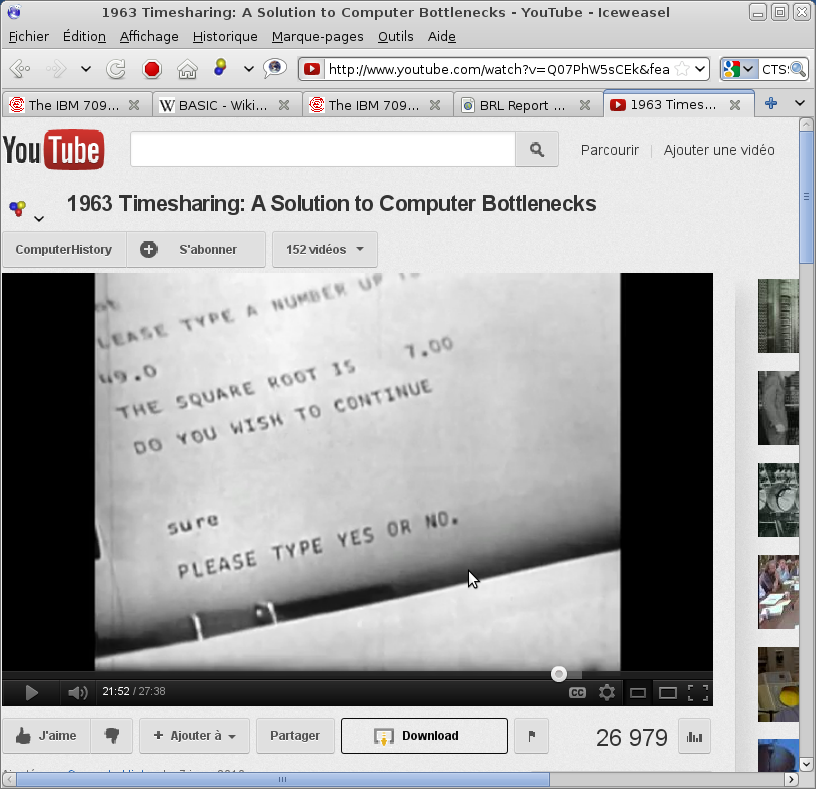
\includegraphics[width=.8\linewidth]{Videos/corbato-demo.png}
\end{center}



\end{multicols}
\emph{
« Hundreds of people will one day be able to use tomorrow's computers simultaneously »} (1963)
\url{http://www.youtube.com/watch?v=Q07PhW5sCEk}
\end{frame}

\begin{frame}
\frametitle{Temps partagé}

Nécessite
\begin{itemize}
\item système de \alert{temps partagé préemptif}
\\
pour empêcher un processus qui boucle de monopoliser la machine
\item\alert{ mémoire virtuelle}
\\
pour disposer d'une mémoire plus grande que la mémoire réelle
\end{itemize}
\end{frame}

\section{Résumé...}

\begin{frame}
\frametitle{En résumé}

\begin{enumerate}
\item un \alert{système d'exploitation} est un programme qui gère des
  ressources : mémoire, périphériques, et ... temps.
\item intermédiaire entre les programmes et le matériel
\item grands principes mis en oeuvre dans les ordinateurs
  commercialisés des années 50 et 60.
\item évolution conjointe avec le matériel et les usages
\end{enumerate}
\vfill
\pause
Quoi de neuf ?
\end{frame}

\begin{frame}
\frametitle{
L'évolution n'est pas terminée !
}
Exemple
\begin{itemize}
\item \alert{miniaturisation} : un ordinateur dans quelques
centimètres cubes.
\item produit grand public : ordinateurs portables,  smartphones
\item mémoire et processeur suffisants pour faire tourner des
applications sur un 
\alert{système multi-tâches} 
\end{itemize}
\alert{Mais...} \pause
\begin{itemize}
\item autonomie électrique ?
\end{itemize}

\alert{Impact sur...}
\pause
\begin{itemize}
\item les matériels
\item les systèmes ?
\end{itemize}
\end{frame}

\begin{frame}
\frametitle{Chapitres du cours}

Dans un système multi-tâches :
\begin{itemize}
\item Gestion des processus 
\item Gestion de la mémoire 
\item Périphériques et systèmes de fichiers
\item ...
\end{itemize}
\end{frame}

\end{document}
